\documentclass[UTF8,zihao=-4,oneside]{ctexart}

\usepackage[a4paper,left=24mm,right=24mm,top=24mm,bottom=22mm]{geometry}
\usepackage{graphicx}
\usepackage{float}
\usepackage{caption}
\usepackage{booktabs}
\usepackage{longtable}
\usepackage{xcolor}
\usepackage{setspace}
\usepackage{titlesec}
\usepackage{hyperref}

\setCJKmainfont{Noto Serif SC}[AutoFakeBold=2]
\setCJKsansfont{Noto Sans SC}[AutoFakeBold=2]
\setmainfont{Arial}
\setsansfont{Arial}

\definecolor{TitleInk}{HTML}{253238}
\definecolor{CaptionInk}{HTML}{6A747A}

\hypersetup{
  colorlinks=true,
  linkcolor=TitleInk,
  urlcolor=TitleInk
}

\setstretch{1.42}
\setlength{\parindent}{2em}
\setlength{\parskip}{0.35em}
\captionsetup{
  font={small,sf},
  labelformat=empty,
  textfont={color=CaptionInk},
  skip=6pt
}

\titleformat{\section}
  {\sffamily\Huge\bfseries\color{TitleInk}}
  {}{0pt}{}
\titleformat{\subsection}
  {\sffamily\Large\bfseries\color{TitleInk}}
  {}{0pt}{}
\titleformat{\subsubsection}
  {\sffamily\normalsize\bfseries\color{TitleInk}}
  {}{0pt}{}

\graphicspath{{../../assets/chapter-01/modern-hanfu-v3/}}

\begin{document}

\section*{一、强健体魄}

\subsection*{精神}

体能在日常生活里近乎隐形，在极端情况下决定你能做什么。

郑州地铁积水持续上涨的高危阶段里（约3至4小时），967人面对同样的条件：没过胸口的冷水，车厢内信号中断、广播失效（据幸存者描述）。有人在这段时间保持清醒，持续帮助旁边的人维持平衡，窗户被破开后协助老人和孩子先撤离。有人更早体力透支，成为需要被照顾的对象。

在胸口深度的冷水里持续站立数小时、保持肌肉协调和清醒判断——这是心肺耐力和肌肉耐力的直接体现，两者都是通过训练可以系统提升的能力。

身体能力的上限，决定了极端条件下你能参与到什么程度。这是这一节的起点。

\subsection*{两套标准的差距}

《国家学生体质健康标准》设计目标是教育评估：筛查学生群体基础运动能力的下限，识别需要干预的个体。测试项目——50米跑、长距离跑、立定跳远、引体向上或仰卧起坐、坐位体前屈——有效测量了它们被设计来测量的能力。

真实场景所需要的能力清单，与标准测试的项目清单只有部分重叠。郑州地铁积水持续上涨的那数小时里，让人能持续帮助他人的能力是：在低温环境下维持肌肉控制的耐力，以及持续协助他人移动所需的上肢和核心力量。这两项都不在《国家学生体质健康标准》的测试项目里。

这本书关注的能力范围，在官方测试项目的边界之外。

\subsection*{可用性标准}

\begin{figure}[H]
  \centering
  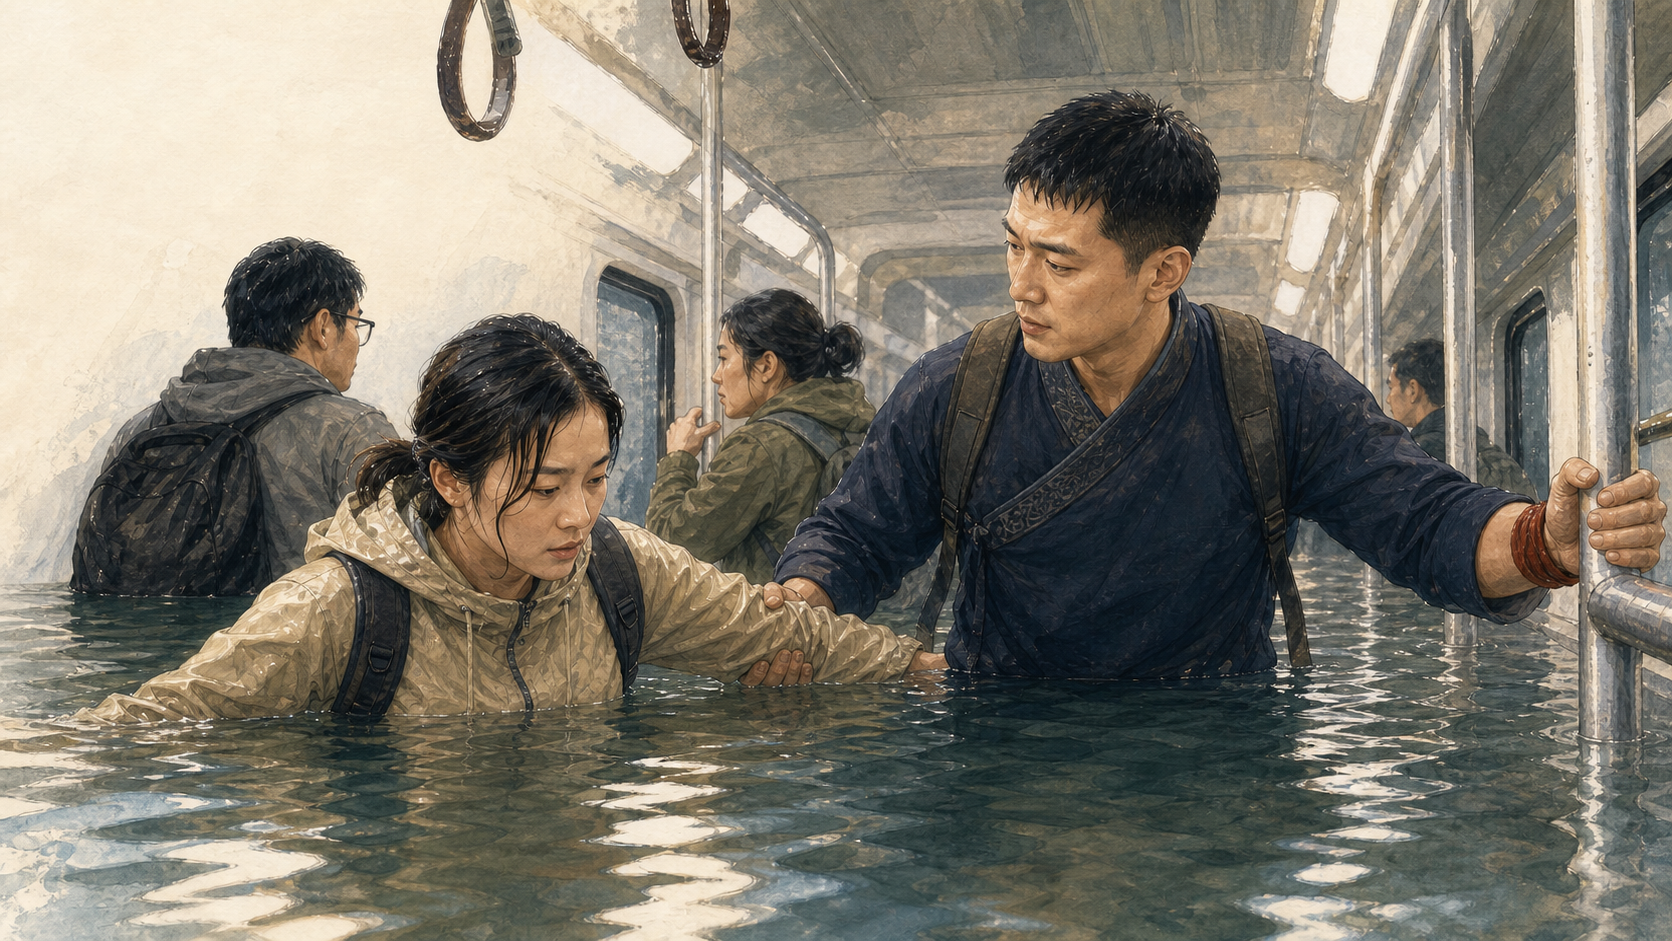
\includegraphics[width=\linewidth]{ch01-hero-flood-modern-hanfu-v3.png}
  \caption{第一章主图：城市洪水中的互助与体能可用性}
\end{figure}

以下是一套以功能为导向的体能评估框架，分三个层级。每个层级对应一种真实场景下的身体需求。

\subsubsection*{第一级：自保}

你的身体，在危机发生的初始阶段，能维持自身运作吗？

测试一：5公里机动能力。在没有提前准备的情况下，以能正常说话的配速跑完或走完5公里，途中不需要停下休息。

测试二：阶梯承压。不停下地爬完10层楼梯，到达顶层时能立即说一句完整的话。

测试三：负重持续行动。背一个装有10到15公斤物品的背包，以正常步行速度持续行走30分钟。

\subsubsection*{第二级：互救}

你的身体，在他人需要时，能提供有效帮助吗？

测试四：拖拽测试。将一个装有约70公斤物品的袋子放在平坦地面上，双手抓住，向后拖行10米，中间不停下。

\begin{figure}[H]
  \centering
  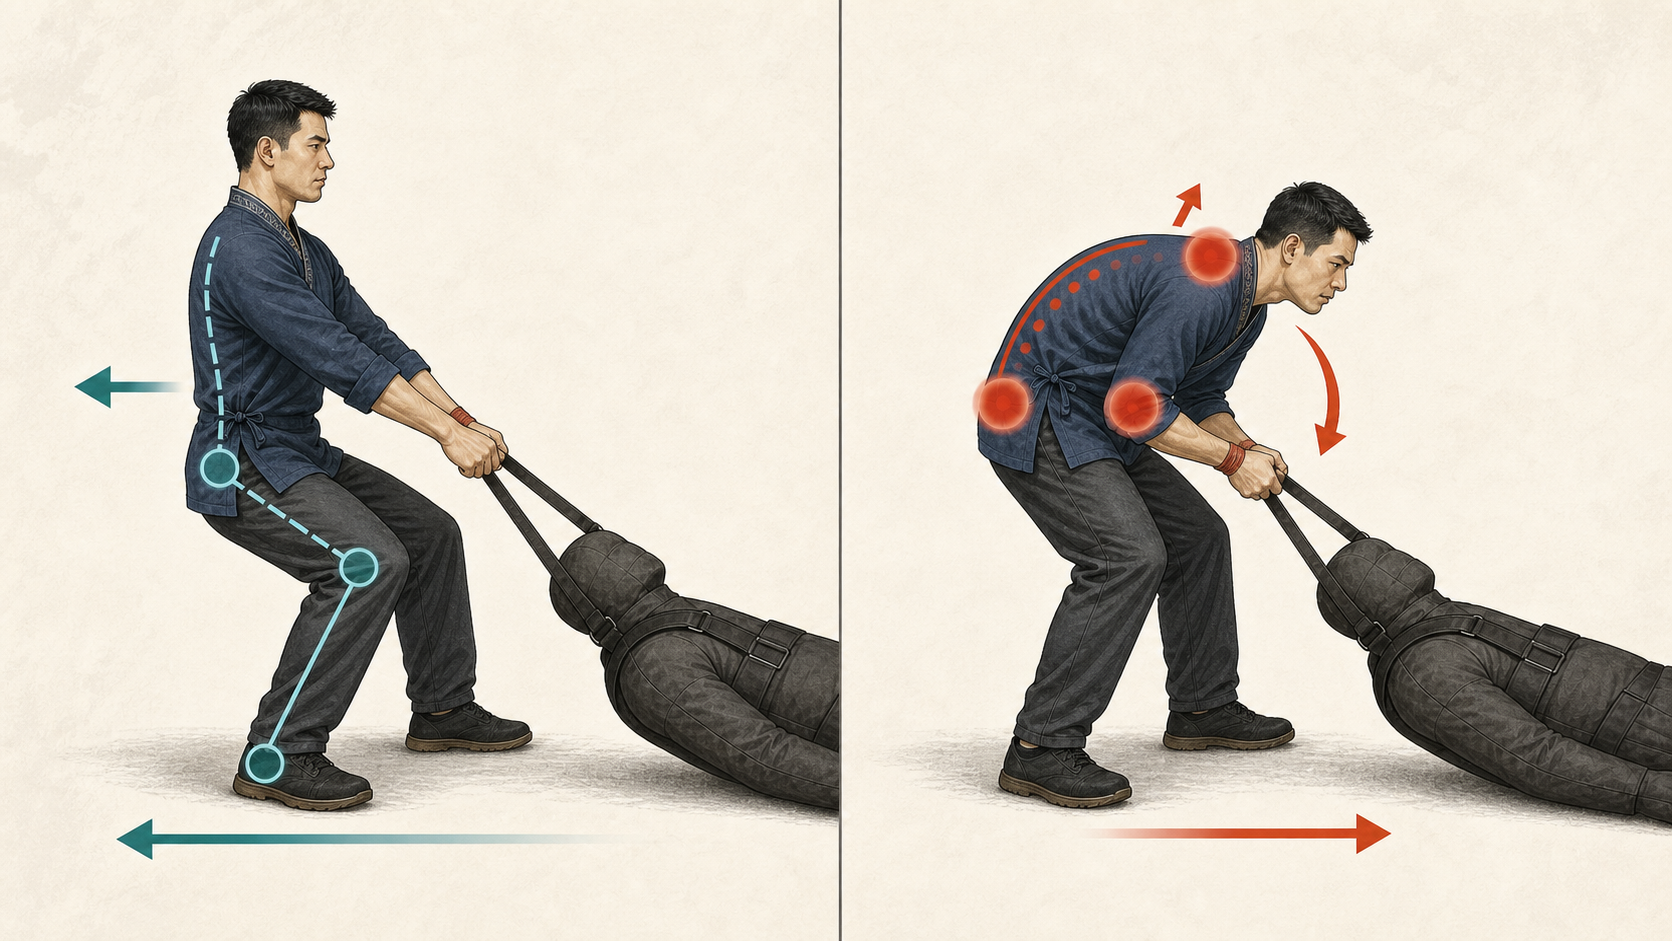
\includegraphics[width=\linewidth]{ch01-rescue-drag-modern-hanfu-v3.png}
  \caption{拖拽测试姿势对比}
\end{figure}

70公斤是中国成年男性的平均体重区间，对应“将一个失去意识的人从危险区域移开”的基础场景。美国消防员候选人体能测试（CPAT）的营救拖拽标准，是将约75公斤的假人拖拽约10.7米。

\subsection*{准备活动}

每次训练前完成热身，是训练计划的组成部分，与正式训练等权重。

\begin{figure}[H]
  \centering
  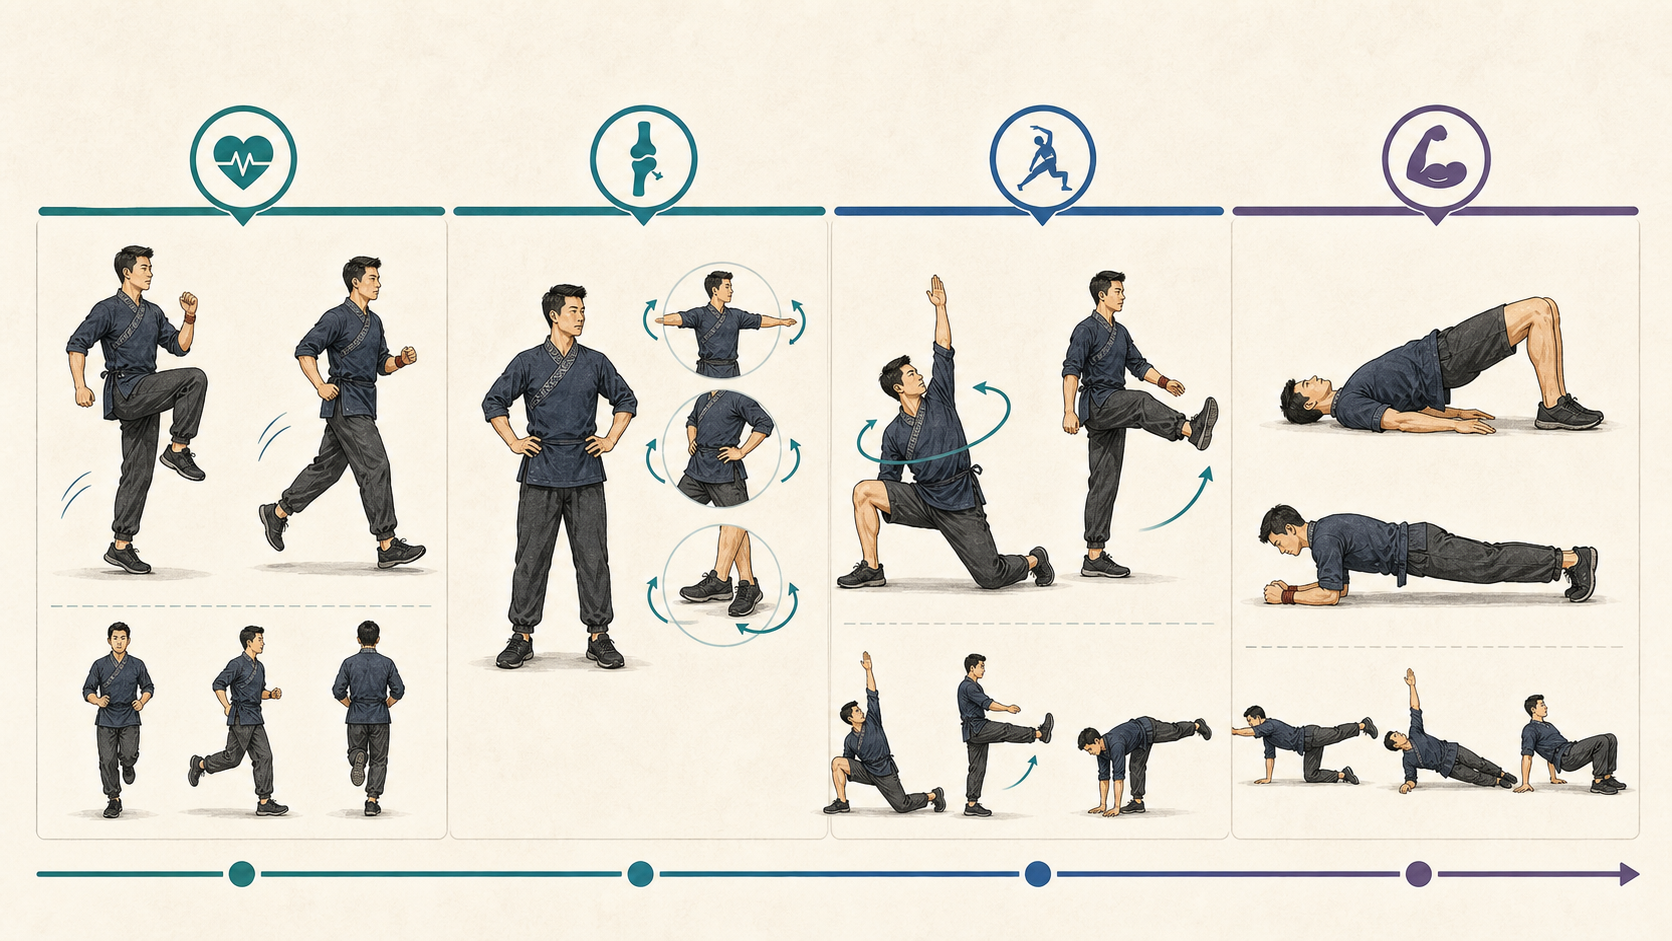
\includegraphics[width=\linewidth]{ch01-warmup-flow-modern-hanfu-v3.png}
  \caption{热身四阶段流程}
\end{figure}

以下是一套完整的动态热身流程，总时长10—15分钟，适用于所有训练日。

\subsubsection*{第三阶段：动态拉伸}

动态拉伸通过运动中的拉伸激活肌肉，适合训练前。静态拉伸放在训练后。

\begin{figure}[H]
  \centering
  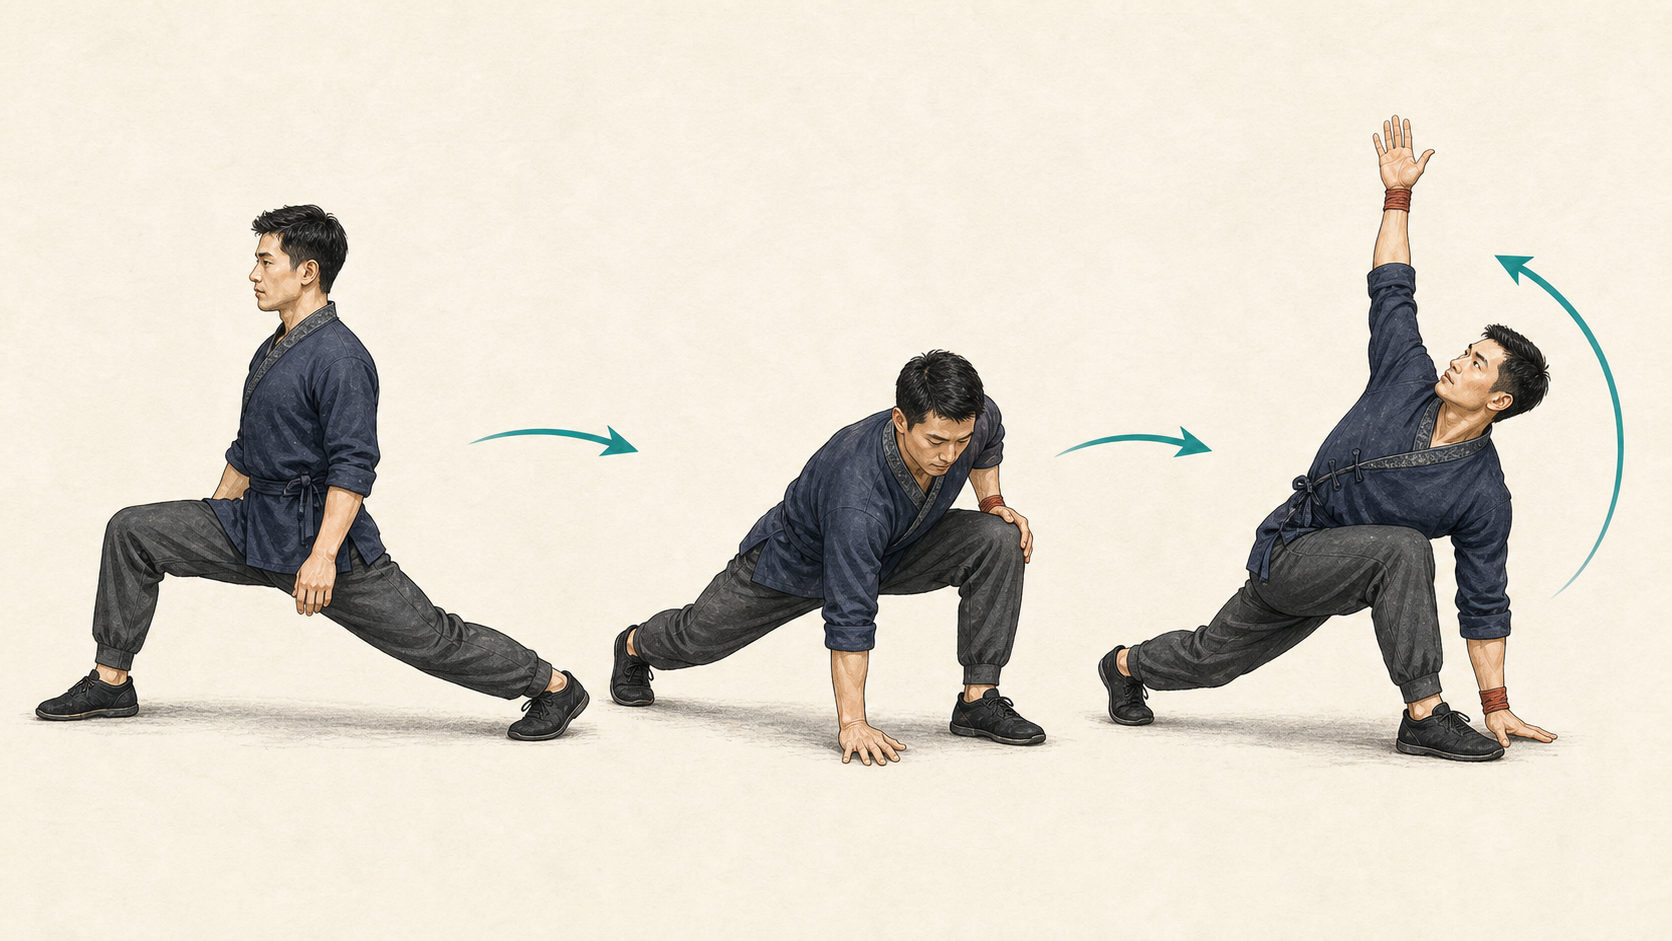
\includegraphics[width=\linewidth]{ch01-lunge-rotation-modern-hanfu-v3.png}
  \caption{弓步加旋转动作分解}
\end{figure}

\subsection*{体能的社会维度}

体能训练有一个不在测试表上的功能。

一起跑过山路，一起在负重状态下找路，一起在体能接近极限时互相告知状态——这个过程建立的，是“我知道这个人在压力下是什么状态”。

\subsubsection*{班组挑战：让弱者的存在变成训练的一部分}

3—6人组成一个班组，完成一个共同的体能任务。团队的成绩，取最后一名到达或完成者的时间。

\begin{figure}[H]
  \centering
  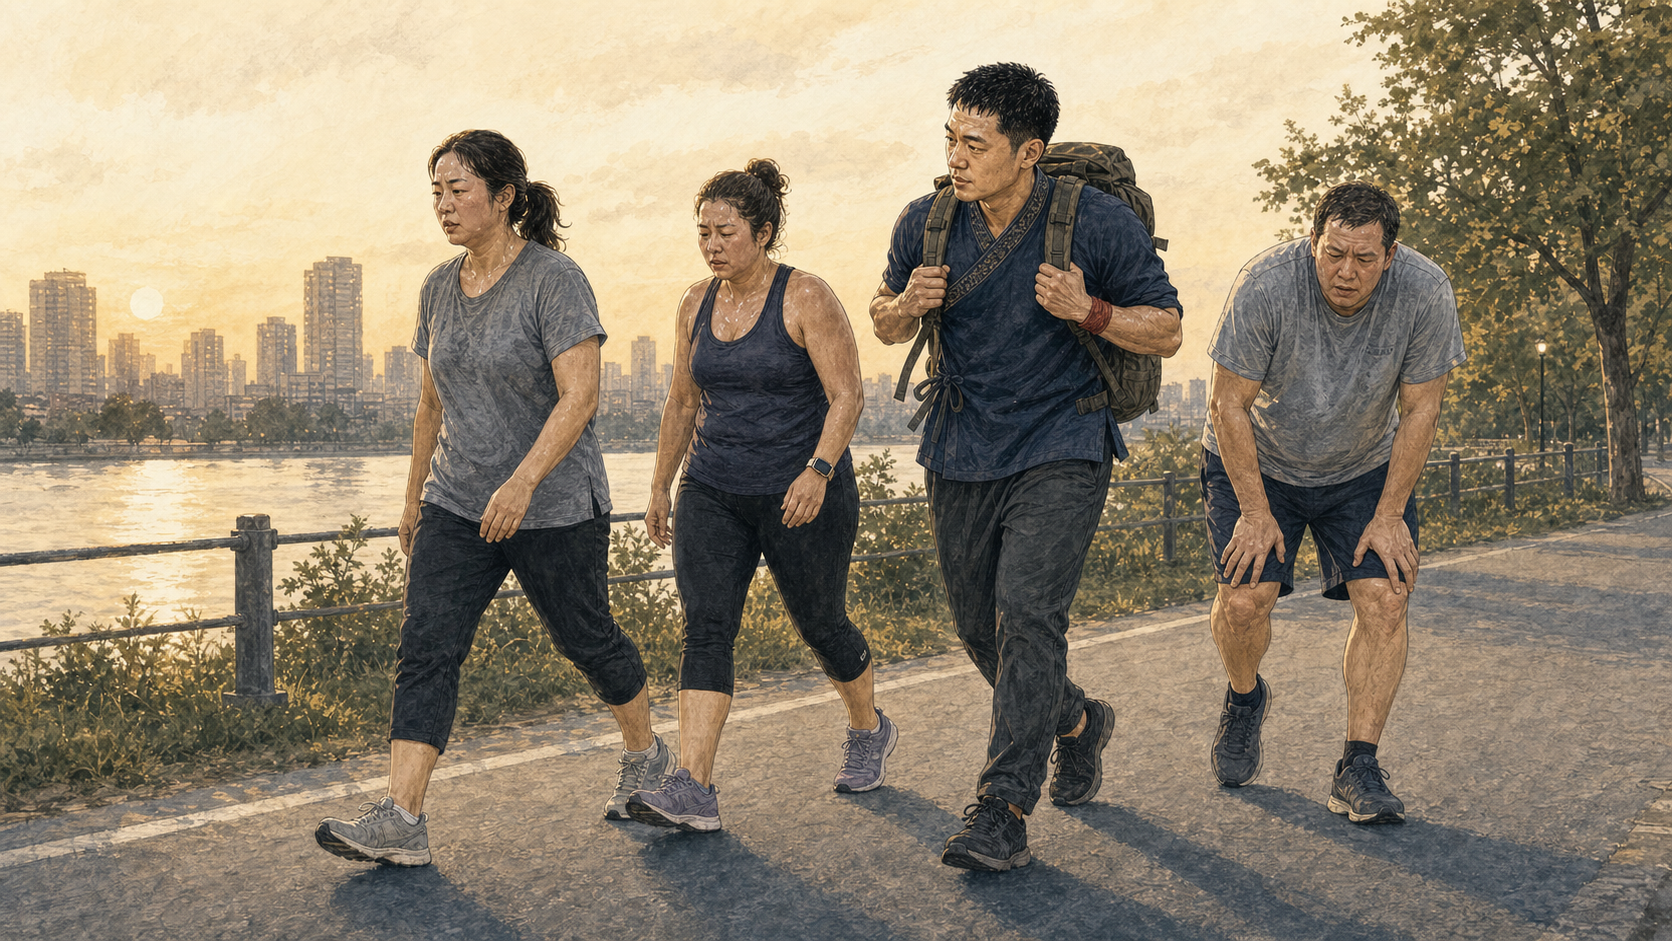
\includegraphics[width=\linewidth]{ch01-team-challenge-modern-hanfu-v3.png}
  \caption{班组挑战：团队按最后一名完成计时}
\end{figure}

在这个规则下，体能最好的成员跑到前面自己完成对团队成绩没有任何贡献。他们的选项变成：放慢步速陪伴较慢的队友；把自己背包里的部分重量转移给体能较弱者；在体能临界点附近用语言激励队友继续。

\end{document}
